% ================================================================
%  ДЗ 1 «Data Detective» — отчёт
%  Компилируется через XeLaTeX (Overleaf: Menu -> Compiler -> XeLaTeX)
% ================================================================

\documentclass[11pt,a4paper,twocolumn]{article}

% ---- Кодировка и шрифты для русского ----
\usepackage{fontspec}
\usepackage{polyglossia}
\setmainlanguage{russian}
\setotherlanguage{english}
\setmainfont{CMU Serif}
\setsansfont{CMU Sans Serif}
\setmonofont{CMU Typewriter Text}
\newfontfamily\cyrillicfonttt{CMU Typewriter Text}

% ---- Остальные пакеты ----
\usepackage[margin=2cm]{geometry}
\usepackage{graphicx}
\usepackage{booktabs}
\usepackage{array}
\usepackage{hyperref}
\usepackage{xcolor}
\usepackage{amsmath}
\usepackage{amssymb}
\usepackage{caption}
\usepackage{float}
\usepackage{parskip}

\setlength{\columnsep}{0.7cm}

\hypersetup{
    colorlinks=true,
    linkcolor=blue!60!black,
    urlcolor=blue!60!black,
    citecolor=blue!60!black,
}

% Моноширинное имя признака; разрешаем перенос строки после «_»
\newcommand{\f}[1]{{\ttfamily\def\_{\textunderscore\allowbreak}#1}}

% В узких колонках даём строкам немного растянуться вместо вылезания за поля
\usepackage{microtype}
\usepackage[raggedright]{titlesec}
\raggedbottom % без растягивания пробелов между абзацами по высоте колонки

% Выравнивание по левому краю с переносами: в узких колонках с моноширинными
% именами признаков это убирает растянутые пробелы внутри строк
\usepackage{ragged2e}
\AtBeginDocument{\RaggedRight}
\captionsetup{justification=RaggedRight, singlelinecheck=false}

% ---- Заголовок ----
\title{
    \vspace{-2cm}
    \textbf{ДЗ 1: Data Detective} \\
    \large Отчёт-расследование
}
\author{
    Safiullin Timur, 415 \\
    \texttt{kaggle-username: \href{https://www.kaggle.com/timursafiullin}{timursafiullin}}
}
\date{\today}

\begin{document}

\maketitle

% ================================================================
\section{Введение}

Нужно предсказать, будет ли деталь с завода бракованной (\f{defect} $=1$), по показаниям оборудования в момент её изготовления. Среди показателей – сенсоры, температура, вибрации, давление и так далее. Ответом является вероятность брака, метрика~-- ROC-AUC. В \f{train} 4025 строк и 19 столбцов (\f{id}, 17 признаков, \f{defect}), в \f{test}~-- 1500 строк без целевой переменной. Брак составляет $30\%$.

В данные намеренно (преподавателем или кем-то ещё) заложены ошибки, и модель на сырых признаках учится на них. Базовая логистическая регрессия даёт CV ROC-AUC $1.000$ и Public Score $0.593$. Найдено семь проблем, которые были последовательно исправлены. Получена итоговая модель~-- логистическая регрессия на исправленных признаках: CV ROC-AUC $0.974 \pm 0.002$, Public Score $0.95562$.

% ================================================================
\section{Обзор данных (EDA)}
\label{sec:eda}

\subsection{Общая статистика датасета}

Все признаки числовые, пропусков (NaN) нет. \f{line\_id}~-- целое число от 1 до 12, у остальных признаков сотни и тысячи уникальных значений. Сводка по признакам~-- в таблице~\ref{tab:eda}.

Сразу видны две странности. В \f{train} 525 строк полностью повторяют другие строки по всем признакам, то есть, имеем дубликаты. При 16 непрерывных признаках случайное совпадение практически невозможно. У \f{temperature} минимум равен $-999$, а медиана~-- $59.8$. Это можно воспринимать как код ошибки датчика температуры. Таких строк тоже 525 ($15\%$).

\begin{table*}[t]
    \centering
    \caption{Признаки после удаления дубликатов (3500 строк в \f{train}). AUC~-- ROC-AUC самого признака как предсказания \f{defect}; KS~-- статистика Колмогорова--Смирнова между \f{train} и \f{test}.}
    \label{tab:eda}
    \footnotesize
    \begin{tabular}{lcccccc}
        \toprule
        \textbf{Признак} & \textbf{AUC} & \textbf{KS} & \textbf{Медиана train} & \textbf{Медиана test} & \textbf{Std train} & \textbf{Std test} \\
        \midrule
        \f{sensor\_a}     & 0.504 & \textbf{0.878} & $-0.03$  & $4.03$   & 2.04   & 0.70 \\
        \f{sensor\_b}     & 0.500 & \textbf{0.455} & $-0.02$  & $-3.26$  & 2.05   & 4.39 \\
        \f{temperature}   & 0.453 & 0.032 & 59.8     & 59.3     & 378.9  & 395.4 \\
        \f{vibration}     & 0.763 & 0.027 & 4.34     & 4.47     & 59.1   & 60.8 \\
        \f{line\_id}      & 0.525 & 0.019 & 6        & 6        & 3.46   & 3.48 \\
        \f{pressure\_bar} & 0.612 & 0.027 & 5.12     & 5.18     & 1.03   & 0.99 \\
        \f{pressure\_psi} & 0.612 & 0.027 & 74.19    & 75.19    & 14.95  & 14.37 \\
        \f{pressure\_pa}  & 0.612 & 0.027 & 511550   & 518350   & 103064 & 99086 \\
        \f{photo\_lux}    & \textbf{1.000} & \textbf{0.299} & 317.4 & 297.7 & 105.9 & 30.4 \\
        \f{aux\_0}        & 0.497 & 0.185 & $-0.88$  & $-0.33$  & 18.42  & 8.98 \\
        \f{aux\_1}        & 0.498 & 0.260 & $-0.08$  & $0.09$   & 2.39   & 7.69 \\
        \f{aux\_2}        & 0.495 & 0.222 & $-0.09$  & $0.03$   & 17.46  & 6.50 \\
        \f{aux\_3}        & 0.503 & 0.132 & $-0.23$  & $-0.26$  & 6.27   & 10.63 \\
        \f{aux\_4}        & 0.487 & 0.019 & $-0.12$  & $-0.09$  & 15.30  & 15.04 \\
        \f{aux\_5}        & 0.511 & 0.305 & $-0.09$  & $-0.14$  & 17.03  & 4.15 \\
        \f{aux\_6}        & 0.484 & \textbf{0.398} & $-0.04$ & $0.28$ & 2.06 & 17.48 \\
        \f{aux\_7}        & 0.516 & 0.304 & $0.04$   & $-0.87$  & 5.11   & 18.67 \\
        \bottomrule
    \end{tabular}
\end{table*}

\subsection{Распределения признаков}

У \f{vibration} очень тяжёлый правый хвост (рис.~\ref{fig:vib}): медиана $4.3$, $99\%$-квантиль $218$, максимум $1485$, коэффициент асимметрии $11.6$. После преобразования $\log(1+x)$ распределение почти симметрично, и это хорошо. Остальные признаки, кроме \f{temperature}, не имеют заметных выбросов. Это тоже хорошо.

\begin{figure}[tb]
    \centering
    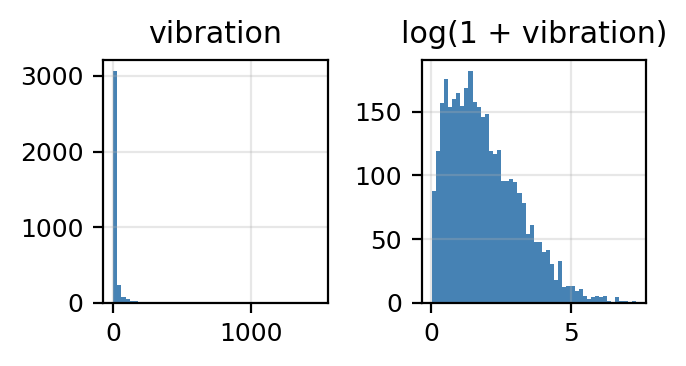
\includegraphics[width=\columnwidth]{figures/vibration.png}
    \caption{\f{vibration} до и после логарифмирования. В исходной шкале почти все значения сжаты у нуля.}
    \label{fig:vib}
\end{figure}

\subsection{Сравнение train и test}

Для каждого признака посчитана статистика KS между \f{train} и \f{test} (табл.~\ref{tab:eda}). У температуры, вибрации, давления и линий распределения совпадают (KS $< 0.035$). Сильнее отличаются следующие три группы:
\begin{itemize}
    \item \f{sensor\_a} и \f{sensor\_b} (рис.~\ref{fig:sensors}). В \f{test} у \f{sensor\_a} все значения положительные, IQR сжат втрое; у \f{sensor\_b} медиана сдвинута на $-3$, IQR вырос вдвое. Корреляция между сенсорами при этом почти та же: $-0.29$ в \f{train}, $-0.24$ в \f{test}.
    \item \f{photo\_lux} (рис.~\ref{fig:lux}): в \f{test} нет значений выше $404$.
    \item \f{aux\_*}: разброс в \f{test} меняется в $0.24 \dots 8.5$ раза, причём медианы остаются около нуля.
\end{itemize}

Проверено и всё вместе через \textit{\href{https://www.kaggle.com/code/carlmcbrideellis/what-is-adversarial-validation}{Adversarial Validation}}. Заставил случайный лес учиться отличать строки \f{train} от строк \f{test}. На сырых признаках он делает это идеально (ROC-AUC $1.00$), после всех исправлений~-- не лучше монетки ($0.505$). Код сюда не стал прикладывать, поскольку сделал через кодинг-агента для проверки гипотезы.

\begin{figure*}[t]
    \centering
    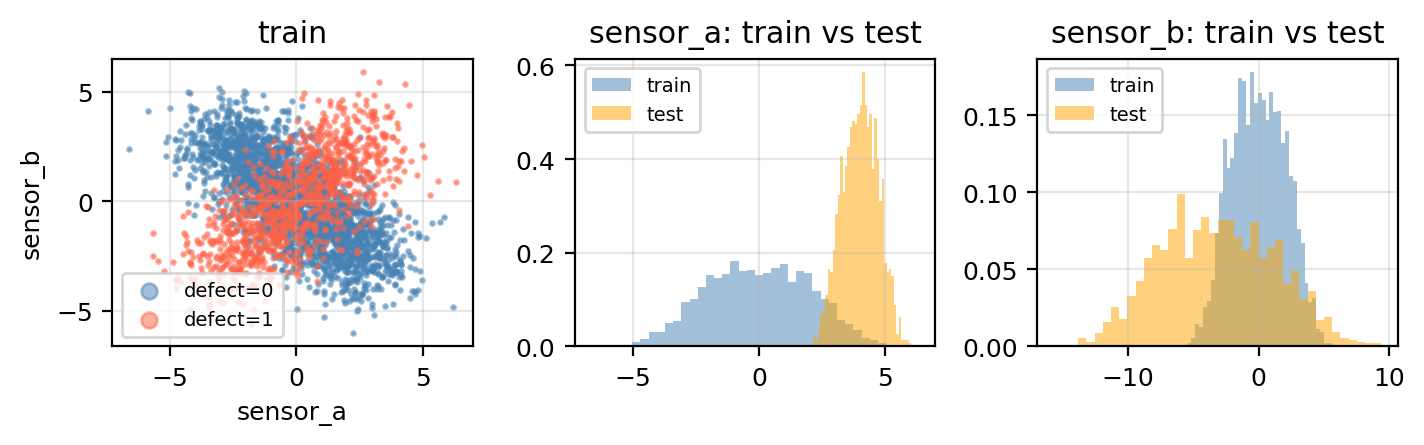
\includegraphics[width=\textwidth]{figures/sensors.png}
    \caption{Слева: сенсоры в \f{train}, цвет~-- класс. Брак сосредоточен в I и III четвертях. Справа: распределения сенсоров в \f{train} и \f{test}.}
    \label{fig:sensors}
\end{figure*}

\subsection{Связь признаков с целевой переменной}

Одиночный ROC-AUC (табл.~\ref{tab:eda}) выделяет \f{photo\_lux} ($1.000$), \f{vibration} ($0.763$) и давление ($0.612$). У сенсоров и \f{aux\_*} он около $0.5$, у \f{line\_id}~-- $0.525$.

Для \f{line\_id} AUC обманчив. Доля брака по линиям (рис.~\ref{fig:lines}) немонотонна. На линиях 3, 7 и 11 она $72 \dots 78\%$, тогда как на остальных~-- $10 \dots 18\%$. Как число \f{line\_id} практически ничего не говорит, но как категория~-- говорит много.

Среди строк с температурой $-999$ брак составляет $78\%$ (407 из 525), при $30\%$ в среднем.

\begin{figure}[tb]
    \centering
    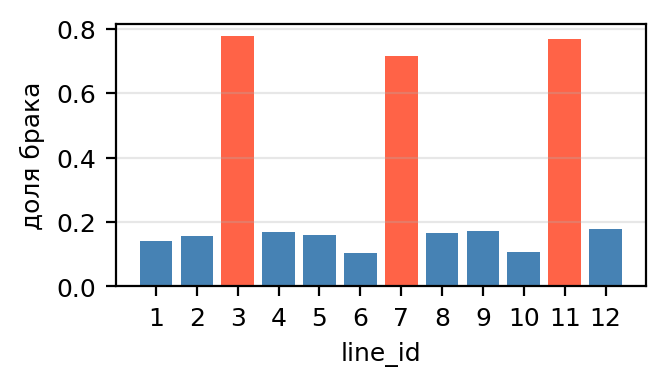
\includegraphics[width=0.85\columnwidth]{figures/lines.png}
    \caption{Доля брака по производственным линиям. Красным~-- линии 3, 7, 11.}
    \label{fig:lines}
\end{figure}

\subsection{Парные наблюдения}

Сенсоры по отдельности бесполезны (AUC $\approx 0.5$), но на парном графике (рис.~\ref{fig:sensors}, слева) видна нелинейная структура типа XOR (т.к. можно достаточно точно предсказать по квадранту). Если знаки \f{sensor\_a} и \f{sensor\_b} совпадают, брак $61 \dots 65\%$; если различаются~-- $10\%$. Произведение \f{sensor\_a}$\cdot$\f{sensor\_b} даёт одиночный AUC $0.894$.

Три столбца давления~-- это одно и то же измерение в барах, psi и паскалях (попарная корреляция $1.000$). Вопрос: зачем?

\subsection{Что показалось подозрительным}

\begin{enumerate}
    \item 525 дубликатов в \f{train}. Копии попадают в разные фолды и завышают CV.
    \item Температура $-999$~-- код ошибки датчика и огромный выброс, так как медиана около $\approx 59$ в обеих выборках.
    \item \f{photo\_lux} разделяет классы почти идеально, а в \f{test} похож только на класс 0~-- вероятно, это утечка.
    \item \f{line\_id}~-- номер линии, но подаётся как число. Не хорошо.
    \item Тяжёлый хвост \f{vibration} портит масштабирование.
    \item Сенсоры. Сигнал только в знаках пары, а в \f{test} знаки сбиты (см. на медиану в  табл.~\ref{tab:eda}, также рис.~\ref{fig:sensors}).
    \item \f{aux\_*}~-- шум с другим масштабом в \f{test}.
\end{enumerate}

% ================================================================
\section{Эксперименты}
\label{sec:experiments}

\subsection{Схема валидации}

Используем \f{StratifiedKFold} на 5 фолдов с перемешиванием (\f{random\_state=42}). Стратификация сохраняет долю брака $30\%$ в каждом фолде. Масштабирование стоит внутри \f{Pipeline}, поэтому \f{StandardScaler} обучается только на обучающей части фолда. Гиперпараметры выбираем только по CV. Public Score смотрим уже после выбора.

Убедиться, что валидация не врёт, помогли три вещи.
\begin{enumerate}
    \item \textbf{Разрыв CV и Public.} На старте CV был $1.000$ при Public $0.593$. То есть, модель опиралась на то, чего нет в \f{test}. По ходу всех исправлений разрыв сократился до $0.02$.
    \item \textbf{Удаление дубликатов до CV.} Если этого не сделать, копия строки оказывается и в обучающем, и в проверочном фолде. Тогда CV проверяет модель на строках, которые она уже видела, и, следовательно, завышает качество.
    \item \textbf{Контроль сдвига.} CV строится только на \f{train} и в принципе не видит, что признак в \f{test} устроен иначе. Поэтому перед обучением ноутбук считает KS по всем признакам модели и выводит те, у которых KS $> 0.1$. В финальной версии таких нет (максимум $0.035$ у \f{sensor\_prod}).
\end{enumerate}

Итоговая таблица по шагам~-- табл.~\ref{tab:exps}. CV в ней посчитан логистической регрессией с \f{C=1}. То есть, без регуляризации.

\begin{table*}[t]
    \centering
    \caption{Эксперименты по порядку: CV ROC-AUC (5 фолдов) и Public Score после каждого шага. $\Delta$~-- изменение Public относительно предыдущего шага.}
    \label{tab:exps}
    \footnotesize
    \begin{tabular}{llccc}
        \toprule
        \textbf{Шаг} & \textbf{Изменение} & \textbf{CV ROC-AUC} & \textbf{Public} & \textbf{$\Delta$ Public} \\
        \midrule
        EXP-000 & базовая логистическая регрессия на всех признаках & $1.000$ & 0.59344 & --- \\
        EXP-001 & удалили дубликаты & $1.000$ & 0.59766 & $+0.00422$ \\
        EXP-002 & $-999 \to$ медиана и индикатор, \textit{только в train} & $1.000$ & 0.39821 & $-0.19945$ \\
        EXP-003 & откат EXP-002; удалили \f{photo\_lux} & $0.799 \pm 0.008$ & 0.76342 & $+0.16576$ \\
        EXP-004 & $-999 \to$ медиана в train и test, без индикатора & $0.764 \pm 0.011$ & 0.76354 & $+0.00012$ \\
        EXP-005 & one-hot для \f{line\_id} & $0.872 \pm 0.017$ & 0.83289 & $+0.06935$ \\
        EXP-006 & $\log(1+\f{vibration})$ & $0.893 \pm 0.014$ & 0.86375 & $+0.03086$ \\
        EXP-007 & калибровка сенсоров по выборке, \f{sensor\_prod} & $0.964 \pm 0.003$ & 0.94359 & $+0.07984$ \\
        EXP-008 & удалили \f{aux\_*} & $0.964 \pm 0.002$ & 0.94638 & $+0.00279$ \\
        EXP-009 & вернули индикатор \f{temperature\_invalid} & $\mathbf{0.974 \pm 0.002}$ & \textbf{0.95562} & $+0.00924$ \\
        \bottomrule
    \end{tabular}
\end{table*}

\subsection{Найденные проблемы и исправления}

\subsubsection{Проблема 1: дубликаты строк}
\textbf{Наблюдение и гипотеза.} 525 строк \f{train} совпадают с другими по всем 17 признакам, метки у копий одинаковые. Строки скопированы при сборке данных: новой информации в них нет, но они завышают CV.

\textbf{Исправление.} Удалили дубликаты по признакам (без \f{id} и \f{defect}), осталось 3500 строк.

\textbf{Эффект.} Public $0.59344 \to 0.59766$. CV остался $1.000$ из-за \f{photo\_lux}.

\subsubsection{Проблема 2: температура $-999$}
\textbf{Наблюдение.} Температура равна $-999$ у $15\%$ строк \f{train} и $17\%$ строк \f{test}. Нормальные значения лежат в диапазоне $31 \dots 87$.

\textbf{Гипотеза.} $-999$~-- код ошибки датчика. Само значение нужно заменить, а факт сбоя может быть полезен, потому что среди таких строк $78\%$ брака.

\textbf{Проверка.} Первая попытка (\textbf{EXP-002}) провалилась, потому что замена была только в \f{train} (раздел~\ref{sec:failures}). В \textbf{EXP-004} заменили $-999$ медианой \f{train} ($61.8$) в обеих выборках. Индикатор тогда убрали: была гипотеза, что связь «$-999 \Rightarrow$ брак» есть только в \f{train}. В \textbf{EXP-009} проверили её без меток. Записи с $-999$ в \f{test} устроены так же, как в \f{train}:

\begin{center}
\small
\begin{tabular}{lcc}
    \toprule
    & \textbf{train} & \textbf{test} \\
    \midrule
    доля $-999$ & 0.150 & 0.167 \\
    медиана \f{vibration}, $-999$ & 9.9 & 10.3 \\
    медиана \f{vibration}, остальные & 3.8 & 3.8 \\
    доля $-999$ на линиях 3/7/11 & 0.289 & 0.323 \\
    доля $-999$ на остальных & 0.104 & 0.115 \\
    \bottomrule
\end{tabular}
\end{center}

Сбой датчика чаще случается на проблемных линиях и при сильной вибрации, и в \f{test} это так же. Значит, индикатор переносится на \f{test}. Всё хорошо.

\textbf{Исправление.} Медиана вместо $-999$ в обеих выборках и бинарный признак \f{temperature\_invalid}.

\textbf{Эффект.} Медиана без индикатора: CV $0.799 \to 0.764$, Public $0.76342 \to 0.76354$. Индикатор: CV $0.964 \to 0.974$, Public $0.94638 \to 0.95562$.

\subsubsection{Проблема 3: утечка через \f{photo\_lux}}
\textbf{Наблюдение и гипотеза.} \f{photo\_lux} один разделяет классы без ошибок (AUC $1.000$, рис.~\ref{fig:lux}), а в \f{test} совпадает с распределением класса 0. Признак, вероятно, измеряется после проверки детали, то есть это утечка. В \f{test} она не работает, и модель будет считать почти все детали годными.

\textbf{Исправление.} Удалили \f{photo\_lux}.

\textbf{Эффект.} CV $1.000 \to 0.799$, Public $0.59766 \to 0.76342$. CV упал, а Public Score вырос на $0.166$. CV завышала именно утечка.

\begin{figure}[tb]
    \centering
    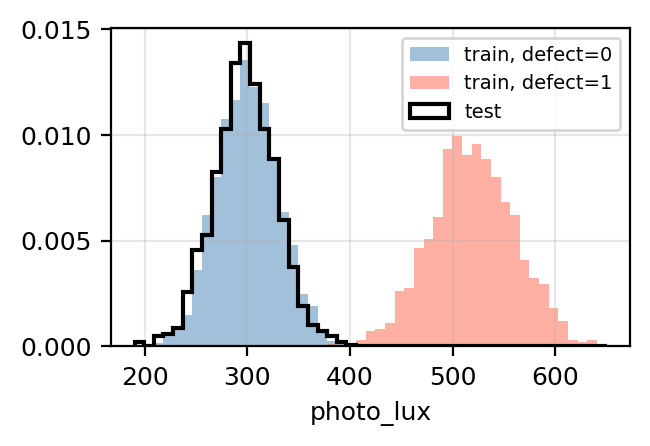
\includegraphics[width=0.85\columnwidth]{figures/photo_lux.png}
    \caption{\f{photo\_lux}: классы в \f{train} не пересекаются, \f{test} похож только на класс 0.}
    \label{fig:lux}
\end{figure}

\subsubsection{Проблема 4: \f{line\_id} как число}
\textbf{Наблюдение и гипотеза.} Доля брака по линиям немонотонна (рис.~\ref{fig:lines}). Один коэффициент при \f{line\_id} описывает только монотонную зависимость от номера, а правило «линии 3, 7, 11 плохие» так не выразить.

\textbf{Исправление.} One-hot кодирование \f{line\_id} (12 бинарных признаков), столбцы \f{test} выровнены по \f{train}.

\textbf{Эффект.} CV $0.764 \to 0.872$, Public Score $0.76354 \to 0.83289$. Коэффициенты модели у линий 3, 7, 11 положительные ($0.55 \dots 0.64$), у остальных отрицательные.

\subsubsection{Проблема 5: тяжёлый хвост \f{vibration}}
\textbf{Наблюдение и гипотеза.} Медиана $4.3$, максимум $1485$ (рис.~\ref{fig:vib}). Несколько десятков огромных значений задают стандартное отклонение $59$. После \f{StandardScaler} основная масса значений $0 \dots 14$ попадает в узкий интервал около нуля, и модель плохо их различает. Удалять большие значения нельзя. Наверное. Это может быть реальная сильная вибрация, и более того, такие значения есть в \f{test}.

\textbf{Исправление.} $\f{vibration} \to \log(1+\f{vibration})$ в обеих выборках. Асимметрия: $11.6 \to 0.8$.

\textbf{Эффект.} CV $0.872 \to 0.893$, Public Score $0.83289 \to 0.86375$.

\subsubsection{Проблема 6: XOR сенсоров и перекалибровка}
\textbf{Наблюдение.} Сенсоры по отдельности не связаны с \f{defect}, но вместе дают XOR (рис.~\ref{fig:sensors}). В \f{test} они сдвинуты и растянуты, но корреляция между ними практически не изменилась.

\textbf{Гипотеза.} Линейная модель не может выучить XOR из двух исходных признаков, ей нужно произведение. Но произведение зависит от знаков, а в \f{test} знаки сбиты: у \f{sensor\_a} все значения положительные. Если сохранилась только форма распределения, датчики перекалибровали, то есть $x_{test} = a x + b$. Тогда приведение каждого сенсора к медиане $0$ и IQR $1$ отдельно в каждой выборке вернёт знаки на место.

\textbf{Проверка.} После калибровки KS между \f{train} и \f{test}: $0.878 \to 0.025$ у \f{sensor\_a}, $0.455 \to 0.016$ у \f{sensor\_b}. Одиночный AUC произведения на \f{train}~-- $0.894$.

\textbf{Исправление.} Калибровка по медиане и IQR отдельно в \f{train} и \f{test}, новый признак \f{sensor\_prod} $=$ \f{sensor\_a}$\cdot$\f{sensor\_b}.

\textbf{Эффект.} CV $0.893 \to 0.964$, Public Score $0.86375 \to 0.94359$~-- самый большой прирост, очень хорошо. У \f{sensor\_prod} самый большой коэффициент в модели ($3.2$ против $1.0$ у \f{vibration}).

\subsubsection{Проблема 7: шумовые \f{aux\_*}}
\textbf{Наблюдение и гипотеза.} У всех \f{aux\_*} одиночный AUC $0.48 \dots 0.52$, у модуля значения тоже, а разброс в \f{test} отличается в $0.24 \dots 8.5$ раза (табл.~\ref{tab:eda}). Сигнала в \f{aux\_*} нет, но модель даёт им небольшие ненулевые веса. На \f{test} эти веса умножаются на значения далеко за пределами \f{train} и добавляют шум в предсказания. На CV этого не видно. Внутри \f{train} сдвига нет.

\textbf{Исправление.} Удалили все \f{aux\_*}.

\textbf{Эффект.} CV $0.964 \to 0.964$, Public Score $0.94359 \to 0.94638$. Изменение видно только на \f{test}, как и ожидалось.


\subsection{Модель}

Во всех экспериментах~-- логистическая регрессия (\f{C=1}) после \f{StandardScaler}, оба шага внутри одного \f{Pipeline}. Нелинейности задачи (XOR сенсоров, плохие линии) вынесены в признаки, поэтому линейной границы достаточно. CV почти не меняется при $C$ от $0.1$ до $100$ и падает только при сильной регуляризации ($C < 0.1$): модель не переобучается, подбирать $C$ точнее нет смысла. Коэффициент при «члене регуляризации» $\frac{1}{C}$.

\subsection{Абляция: вклад каждого исправления}

Из полного набора исправлений убирали по одному и считали CV ROC-AUC (табл.~\ref{tab:ablation}). Public для каждого варианта не считали, чтобы не тратить сабмиты, потому что было ограничение на их число. Поэтому таблица не показывает исправления, которые касаются только \f{test}: калибровку сенсоров по выборке и удаление \f{aux\_*}. Их эффект на Public~-- в табл.~\ref{tab:exps}.

\begin{table}[H]
    \centering
    \caption{CV ROC-AUC логистической регрессии при удалении одного исправления. $\Delta$~-- изменение относительно полного набора. Рост CV означает, что без исправления CV завышен.}
    \label{tab:ablation}
    \footnotesize
    \begin{tabular}{lcc}
        \toprule
        \textbf{Убрано} & \textbf{CV ROC-AUC} & \textbf{$\Delta$} \\
        \midrule
        (ничего)                  & $0.974 \pm 0.003$ & --- \\
        \midrule
        удаление дубликатов       & $0.975 \pm 0.005$ & $+0.001$ \\
        удаление \f{photo\_lux}   & $1.000 \pm 0.000$ & $+0.026$ \\
        $-999 \to$ медиана        & $0.971 \pm 0.001$ & $-0.004$ \\
        индикатор $-999$          & $0.964 \pm 0.003$ & $-0.010$ \\
        one-hot \f{line\_id}      & $0.956 \pm 0.003$ & $-0.019$ \\
        $\log(1+\f{vibration})$   & $0.970 \pm 0.004$ & $-0.004$ \\
        \f{sensor\_prod}          & $\mathbf{0.927 \pm 0.009}$ & $\mathbf{-0.047}$ \\
        удаление \f{aux\_*}       & $0.974 \pm 0.003$ & $0.000$ \\
        \bottomrule
    \end{tabular}
\end{table}

% ================================================================
\section{Что не сработало}
\label{sec:failures}

\textbf{Исправление температуры только в train (EXP-002).} Заменил $-999$ медианой и добавил индикатор, но только в \f{train}. В \f{test} остались $-999$, а модель видела температуры в диапазоне $31 \dots 87$. Коэффициент при температуре положительный, поэтому строки с $-999$ получили почти нулевую вероятность брака и ушли в самый низ ранжирования, хотя в \f{train} среди таких строк $78\%$ брака. Public Score упал до $0.398$, то есть ниже $0.5$. CV этого не показал, потому что считался на исправленном \f{train}. Вывод таков: любое преобразование нужно применять к обеим выборкам одним и тем же кодом.

\textbf{Отказ от индикатора (EXP-004).} После EXP-002 я решил, что индикатор «опасен»: в \f{train} $78\%$ строк с $-999$ бракованные, а я не знал, сохраняется ли это в \f{test}. Убрали индикатор~-- CV упал с $0.799$ до $0.764$. Позже сравнил профиль записей с $-999$ в \f{train} и \f{test} без меток (Проблема 2), увидел одинаковую картину и вернул индикатор (EXP-009): $+0.009$ на Public Score. Ошибка была в том, что гипотезу о \f{test} я не проверил.

% ================================================================
\section{Выводы}

\textbf{Что было не так с данными.} Семь проблем четырёх видов.
\begin{itemize}
    \item Ошибки в данных: дубликаты строк, код ошибки $-999$ в температуре.
    \item Утечка: \f{photo\_lux} знает ответ в \f{train} и не знает в \f{test}.
    \item Сдвиг между \f{train} и \f{test}: перекалиброванные сенсоры и \f{aux\_*} с другим масштабом.
    \item Признаки в неудобном для модели виде: номер линии как число, тяжёлый хвост \f{vibration}, XOR сенсоров, который линейная модель не видит без произведения.
\end{itemize}

\textbf{Что помогло, а что нет.} Больше всего дали удаление \f{photo\_lux}, калибровка сенсоров с \f{sensor\_prod} и one-hot линий ($+0.166$, $+0.080$ и $+0.069$ на Public). Остальные исправления дали $+0.003 \dots 0.031$. Ошибочными были исправление только в \f{train} (EXP-002) и отказ от индикатора (EXP-004). Удаление копий давления ничего не изменили.

\textbf{Что я вынес из задания.}
\begin{itemize}
    \item \textbf{Идеальный CV~-– это повод искать ошибку.} CV $1.000$ на старте означал утечку, а не то, что у нас хорошая модель. Если результат слишком хорош, то есть повод усомниться. Обязательно нужно посмотреть, на что опирается модель.
    \item \textbf{Данные важнее модели.} Public Score в итоге вырос с $0.59$ до $0.956$, а модель при этом всё время оставалась логистической регрессией. Какие вводные – такой и выход, соответственно. Обязательно нужно проводить анализ данных, чистить их от мусора, приводить в порядок.
    \item \textbf{Записывать всё, что делаешь.} Я менял по одному и записывал CV и Public Score после каждого шага. И поэтому было видно, что дало каждое исправление, и тот же EXP-002 легко было откатить. Если ты делаешь одну работу долгое время, ты забываешь, зачем сделал то или иное действие, зачем в моменте принял то или иное решение. Ведение «дневника» дает возможность не держать всю историю в голове.
\end{itemize}

\medskip
\textbf{Воспроизведение.} Итоговый сабмит получается за один запуск ноутбука \mbox{\f{timur\_safiullin\_1hw.ipynb}}. Он скачивает данные через Kaggle API, применяет все исправления, считает CV и сохраняет \f{submission.csv}. Историю того, как я решал задание, можно посмотреть по коммитам в GitHub – https://github.com/timursafiullin/ml-dafe

\medskip
\textbf{Использование ИИ.} В ходе работы над заданием я пользовался помощью таких LLM, как ChatGPT и Claude. Я спрашивал у них, например, как работает утечка данных, почему то или иное решение не сработало, почему это дало маленький прирост к Score и другие глупые вопросы. Также я использовал агентов для кодинга, чтобы быстро проверять гипотезы. Например, я знаю, что если обучающая и тестовая выборка очень схожи, данные повторяются, то это завышает результаты модели. Однако я не знал, как выразить эту схожесть математически и как её проверять (помимо наличия дубликатов). Я нашёл, что есть Adversarial Validation, но не хотел в это углубляться, поэтому попросил у ИИ реализацию. Это позволило мне очень быстро проверить гипотезу. Также, мне было лень заниматься форматированием отчёта, поэтому я дал ИИ доступ к своему «дневнику», который я вёл в ходе работы, и дал доступ к решению. На основе них он сформировал структуру отчёта, вставил картинки и избавил меня от скучной работы с форматированием в LaTeX.

\end{document}
